% Capa com imagem de fundo usando TikZ
\documentclass{article}

\usepackage[dvipsnames]{xcolor}
\usepackage{tikz}
\usetikzlibrary{calc}
\usepackage{anyfontsize}
\usepackage{sectsty}
\usepackage{graphicx} % <-- necessário para \includegraphics

\begin{document}
\pagestyle{empty}

\begin{tikzpicture}[overlay,remember picture]

% --- IMAGEM DE FUNDO (cobre toda a página) -------------------------------
\node[anchor=center, inner sep=0] at (current page.center)
{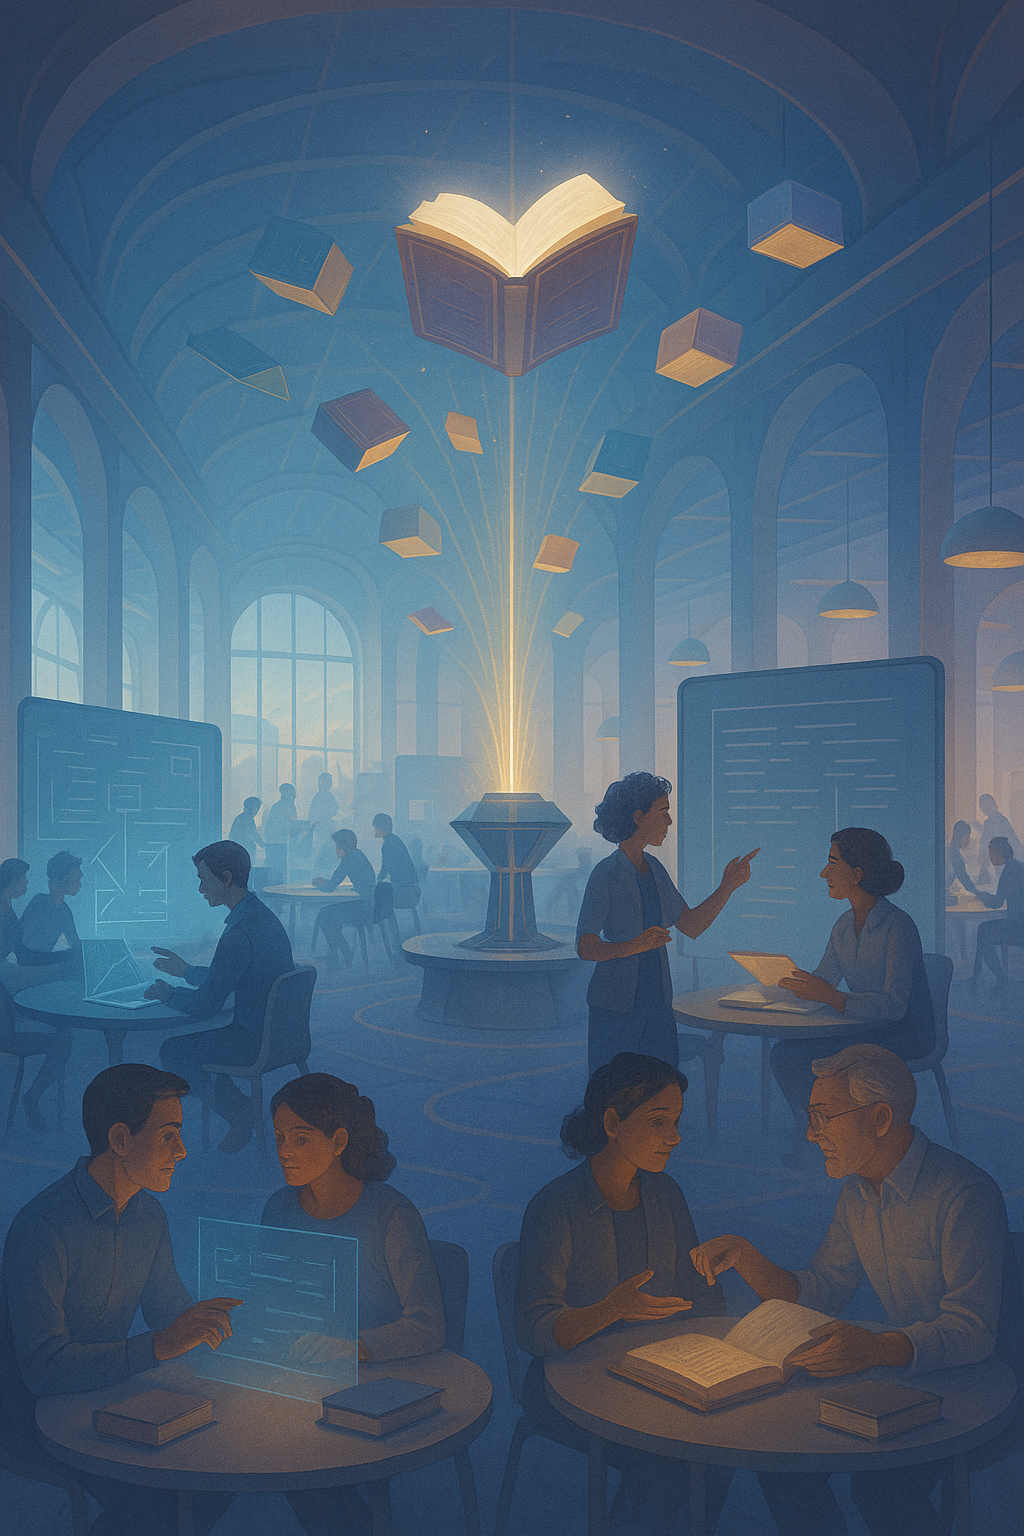
\includegraphics[width=\paperwidth,height=\paperheight]{maquina}};

% (Opcional) Véu para aumentar legibilidade do texto sobre a foto
\fill[black, opacity=0.15]
  (current page.south west) rectangle (current page.north east);


% --- ANO/EDIÇÃO ----------------------------------------------------------
\draw[ultra thick,gray]
($(current page.center)+(5,2)$) -- ++(0,-3cm) 
node[midway, left=0.25cm, text width=5cm, align=right, black!75]
{{\fontsize{25}{30}\selectfont \bf Número 7 \\[10pt] Dezembro}}
node[midway, right=0.25cm, text width=6cm, align=left, orange]
{{\fontsize{72}{86.4}\selectfont 2025}};

% --- TÍTULO --------------------------------------------------------------
\node[align=center] at ($(current page.center)+(0,-5)$)
{
{\fontsize{60}{72}\selectfont \bfseries GESCONS} \\[1cm]
{\fontsize{16}{19.2}\selectfont \textcolor{RoyalBlue}{\bf REVISTA DA ASSOCIAÇÃO INTERNACIONAL EDITARES}}\\[3pt]
};

% --- LOGO ---------------------------------------------------------------
\node at ($(current page.south)+(0,3cm)$)
{
\includegraphics[width=3cm]{Logo-Editares-com-Marca-Registrada}};

\end{tikzpicture}
\end{document}
